\section{Complete source-level results}
\begin{table}[h]
\centering\scriptsize
\begin{tabular}{lrrrrr}
\toprule
Source & Laya EN & Laya Multi & Llama & Qwen & Jev \\
\midrule
ag\_news & 94.3 & 92.4 & 88.9 & 86.8 & 88.6 \\
emotion & 59.1 & 53.0 & 50.5 & 54.8 & 59.0 \\
banking77 & 55.3 & 51.2 & 54.1 & 66.8 & 79.9 \\
massive\_en & 54.1 & 42.3 & 57.2 & 66.3 & 77.5 \\
massive\_zh & 30.4 & 33.2 & 53.5 & 62.6 & 76.0 \\
boolq & 84.6 & 77.7 & 64.8 & 83.5 & 92.6 \\
boolq\_choice & 83.6 & 77.4 & 68.7 & 83.3 & 92.2 \\
xnli\_en & 86.0 & 81.7 & 46.2 & 78.7 & 85.9 \\
xnli\_zh & 61.5 & 74.3 & 40.5 & 69.1 & 73.6 \\
turtlebench & 42.6 & 41.6 & 42.2 & 44.2 & 74.0 \\
sst5 & 34.6 & 29.5 & 32.0 & 45.7 & 56.5 \\
sst5\_choice & 49.6 & 35.6 & 42.2 & 43.9 & 55.9 \\
prompt\_injections & 70.7 & 57.8 & 62.9 & 63.8 & 76.7 \\
aegis2\_prompt & 49.6 & 57.1 & 66.8 & 72.7 & 82.4 \\
typed\_decisions & 36.4 & 34.9 & 51.2 & 55.5 & 73.9 \\
JB: original & 70.8 & 41.7 & 75.0 & 83.3 & 98.6 \\
JB: easy & 95.8 & 89.6 & 100.0 & 100.0 & 100.0 \\
JB: hard & 29.7 & 32.4 & 34.2 & 46.8 & 72.1 \\
ReflexBench & 58.9 & 46.3 & 60.0 & 84.2 & 93.7 \\
JL: triage & 62.5 & 55.7 & 75.6 & 80.0 & 90.0 \\
JL: moderation & 67.8 & 48.4 & 89.0 & 77.5 & 92.7 \\
JL: routing & 64.2 & 51.1 & 61.3 & 83.7 & 88.8 \\
JL: claims & 90.0 & 80.0 & 61.7 & 98.7 & 100.0 \\
JL: reviews & 70.7 & 42.3 & 83.0 & 87.0 & 87.7 \\
JL: guard & 60.6 & 33.2 & 88.0 & 83.2 & 93.8 \\
JL: multilingual & 57.8 & 62.5 & 94.5 & 98.4 & 100.0 \\
clinc150\_oos & 55.7 & 64.8 & 55.2 & 67.8 & 89.5 \\
JL: needle & 50.2 & 47.4 & 77.9 & 87.8 & 95.2 \\
\bottomrule
\end{tabular}

\caption{All 28 main suites, in fixed taxonomy order. Entries are percentage reference agreement; synthetic/authored sources retain their respective reference semantics. These rows are not independent benchmarks and are not averaged. Failure cases remain in denominators. Full per-source cluster intervals, type/language slices and provenance are provided by the machine-readable artifact.}
\end{table}
\clearpage
\begin{figure}[p]
\centering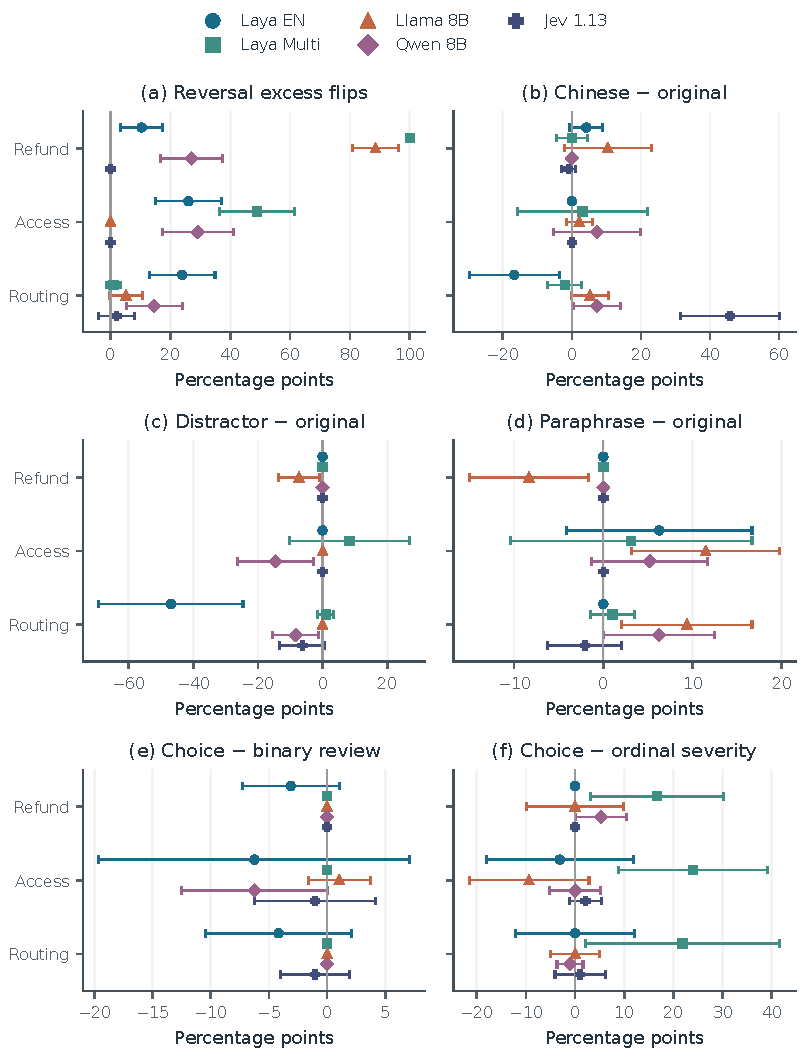
\includegraphics[width=.99\linewidth,height=.85\textheight,keepaspectratio]{figures/fig_confirmation.pdf}
\caption{All six predeclared fresh-policy effects, with 96 base clusters per policy. Whiskers are simultaneous 95\% intervals within the six-effect family of each model/policy, using 10,000 bootstrap draws stratified by generator seed. They do not provide paper-wide coverage. Panel (a) measures excess action flips; (b)--(f) measure correctness differences for the stated primitive. Zero-variance intervals are descriptive, not proof of invariance. Programmatic references follow visible policies. Chinese policy/question/criteria text is authored; structural field and label IDs remain in English.}
\label{fig:confirmation}
\end{figure}
\clearpage
\begin{figure}[p]
\centering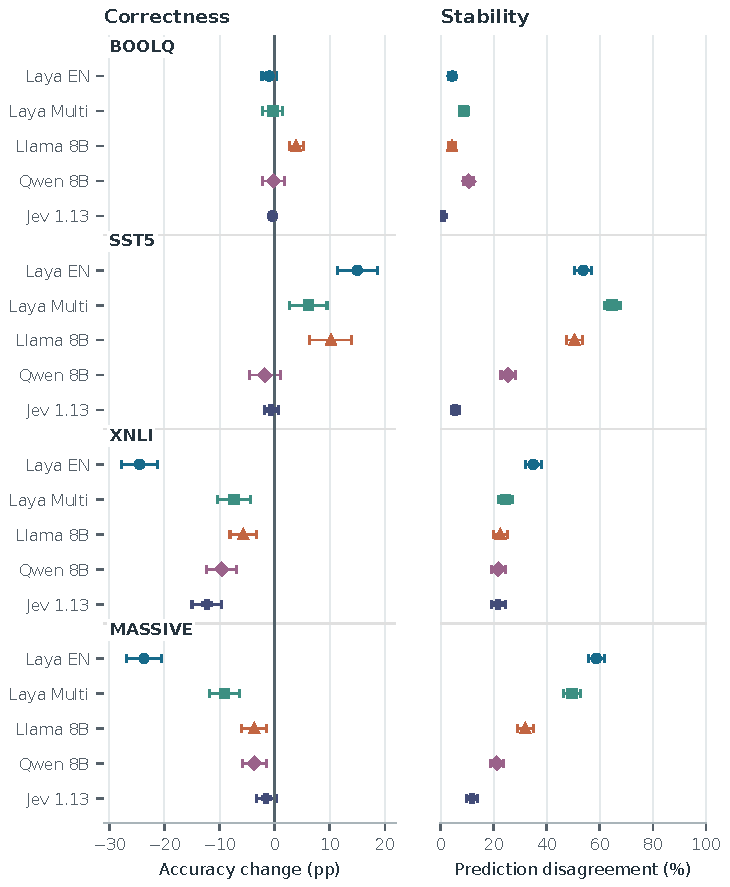
\includegraphics[width=.96\linewidth]{figures/fig_paired.pdf}
\caption{Exploratory paired interface contrasts against dataset-provided references on 1,000 aligned states per task: BoolQ choice minus noul, SST5 choice minus score, and Chinese minus English for XNLI and MASSIVE. Left: accuracy change; right: canonicalized prediction disagreement. Whiskers are pointwise 95\% paired state-cluster bootstrap intervals (10,000 draws). Canonical label mappings are recorded explicitly; no marginal-CI subtraction is used.}
\label{fig:paired}
\end{figure}
\clearpage
\begin{figure}[p]
\centering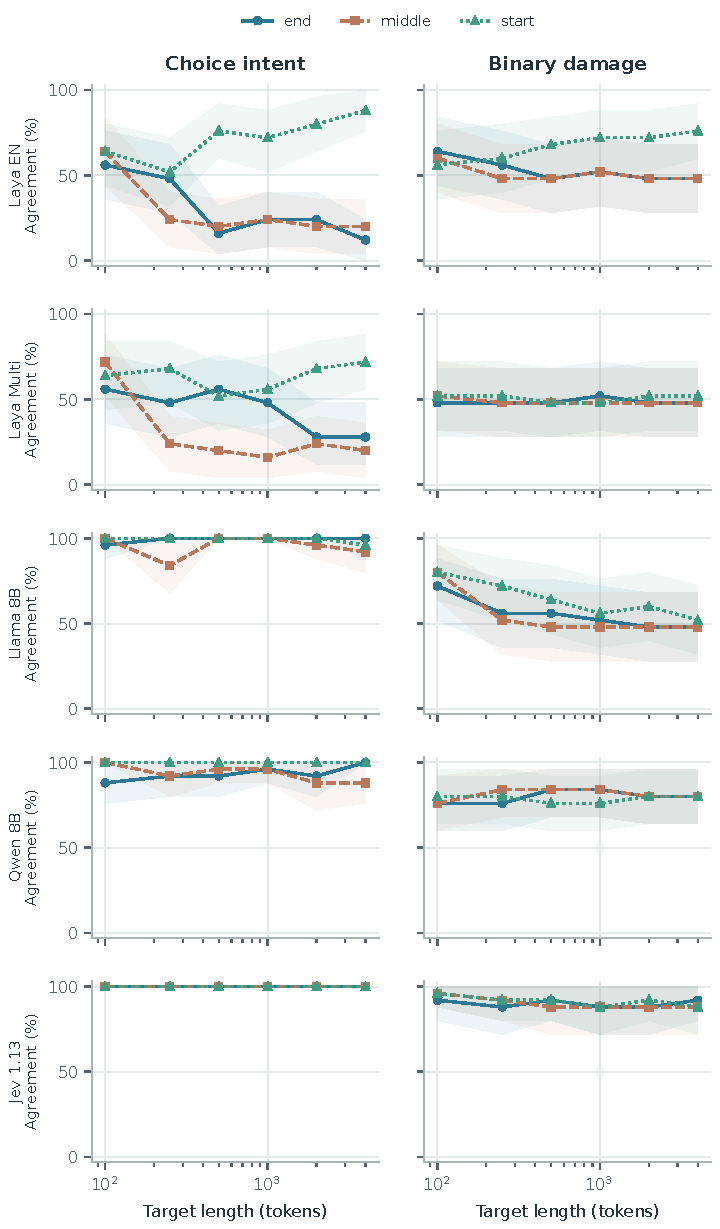
\includegraphics[width=.93\linewidth,height=.84\textheight,keepaspectratio]{figures/fig_context.pdf}
\caption{Programmatic needle reference agreement by source target length, insertion position and question. Rows identify models; left/right columns are the choice intent and binary damage questions. Each point uses 25 original needle clusters; shaded pointwise 95\% cluster intervals resample those originals. Source length targets are not identical tokenizer token counts. The two primitives need not share the same context trend.}
\label{fig:context}
\end{figure}
\clearpage
\begin{figure}[p]
\centering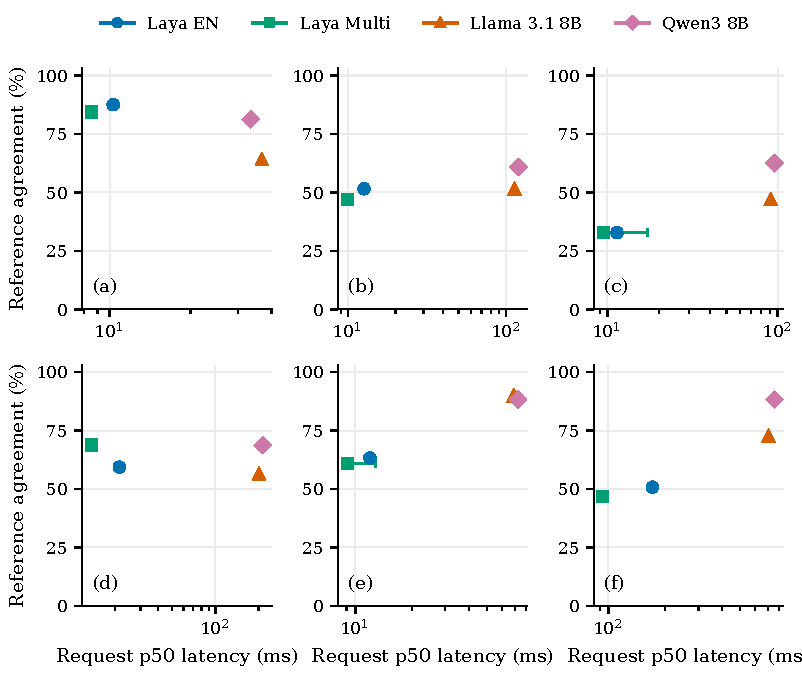
\includegraphics[width=.99\linewidth]{figures/fig_operational.pdf}
\caption{Resident-GPU quality/latency observations on six named workloads. Each stratum has the same 64 measured states across local models. BoolQ, Banking77, MASSIVE and CLINC150 use dataset references; the two needle workloads use programmatic references. Horizontal bars are 95\% bootstrap intervals for the median of eight round p50 latencies; vertical coordinates are median reference agreement over repeated fixed states, not a new population-accuracy estimate. Jev's hosted latency is excluded because its measurement boundary differs. No cross-workload frontier is drawn.}
\label{fig:operational}
\end{figure}
\begin{figure}[p]
\centering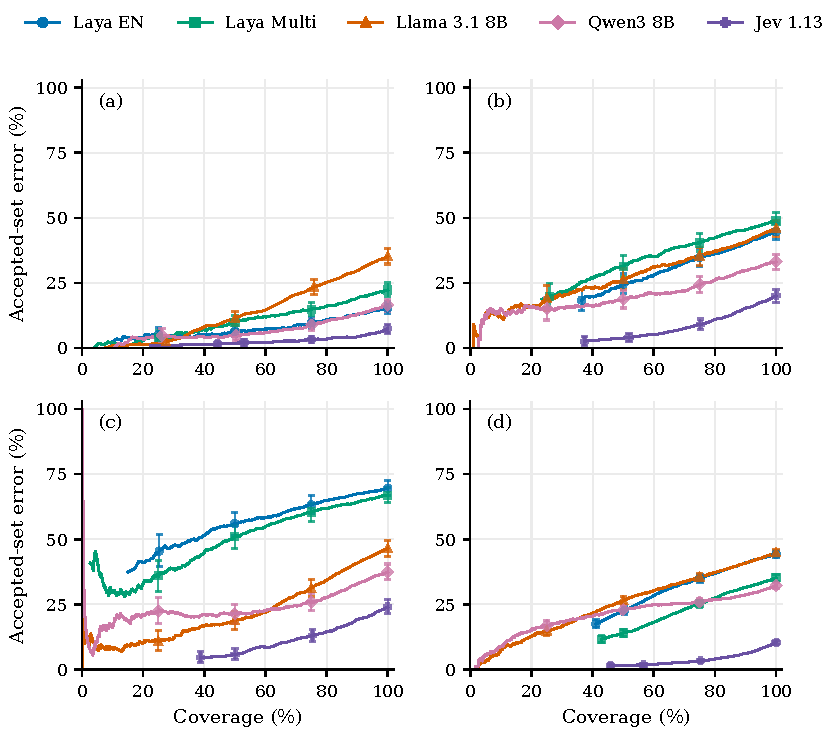
\includegraphics[width=.99\linewidth]{figures/fig_selective.pdf}
\caption{Maximum-probability selective error on (a) BoolQ, (b) Banking77, (c) MASSIVE Chinese and (d) CLINC150 with OOS (1,000, 1,000, 1,000 and 5,500 states). Ties are accepted together. Markers identify realized coverage at nominal 25/50/75/100\% landmarks; intervals resample accepted state clusters conditional on the displayed threshold. Native and candidate-code probability semantics remain distinct. Curves describe the observed test set and do not validate a deployment threshold.}
\label{fig:selective}
\end{figure}
\clearpage
\section{Natural-domain sampling and reference validity}
\label{app:domain-validity}
The separate legal and scientific diagnostic is deliberately balanced for paired sensitivity analysis, not a claim of natural prevalence. ContractNLI has 123 test contracts and 2,091 annotated document--hypothesis decisions, of which 220 are contradictions. The 16,000-character cap removes 24 contracts, disproportionately SEC-HTML files (13/23), versus 7/76 PDFs and 4/24 SEC-text files. The frozen 144 pairs span 91 contracts and contain 48 examples of each of the three labels; 43 of its 48 contradiction cases use four of the 17 fixed hypothesis IDs. To quantify that prior without test-label training, we compute the modal label for each hypothesis on the official 423-contract training split and apply the resulting ID-only lookup to the frozen sample: 82/144 = 56.9\% reference agreement (descriptive 95\% contract-cluster interval [49.3, 64.3]). The same lookup reaches 1,379/2,091 = 65.9\% on the full official test set, illustrating how the frozen class balance changes the question. This supervised label prior is not a fair zero-shot model baseline and does not prove any system uses the shortcut. Neither the cap nor the balanced label mixture supports a prevalence-weighted comparison with ContractNLI's published full-test scores. The observed correctness and reversal effects apply to complete selected contracts and their specified hypotheses only.

SciFact's cited-positive subset contains 120 claim--abstract pairs from 120 distinct claims but only 111 distinct abstracts. It samples 60/64 eligible contradiction claims and 60/124 eligible support claims, so labels are balanced but claim creation mechanisms and source-paper repetition are not. The 112 development-set claims without positive evidence are excluded; the experiment neither assigns them a no-information target nor measures retrieval. Claim-cluster intervals in Figure~\ref{fig:natural-domains} account for claim identity, not shared-abstract dependence. Re-clustering on the 111 abstracts gives nearly identical descriptive intervals: Qwen's reversal accuracy change is $-6.7$ points with claim-cluster interval $[-12.5,-0.8]$ and abstract-cluster interval $[-12.7,-0.8]$; all five alternatives are recorded in the companion analysis. The supplied title and full abstract are visible, while evidence sentence indices and references are not. No local full-input audit can verify hosted server tokenization.

The first hosted attempt at this frozen experiment stopped after 216 requests when one HTTP-200 response selected a different option from its own maximum-probability option. Its append-only journal is retained as a separate aborted run. The primary Jev record is a fresh 792-request execution with an explicitly versioned runner that records such invalid typed outputs without silently selecting an alternative; no invalid decision occurred in that complete execution. This deviation is not used to replace a failed pair in the primary run. Source-text redistribution is separately governed by ContractNLI and SciFact/S2ORC notices in \texttt{research/domain\_expansion\_v1/DATA\_LICENSES.md}; the local source-containing freeze is not shipped in Git.

\paragraph{Three-class SciFact source and input audit.}\label{app:scifact3-audit}
We reconstructed the labeled development claims and complete abstracts from the official SciFact archive, binding archive, source-file, preparer, frozen-request and raw-output SHA-256 hashes in the companion artifact. Among 300 claims and 5,183 corpus abstracts, 340 citation-list occurrences reduce to 339 unique claim--document pairs because claim 1245 repeats one cited ID. The resulting pair counts are 138 SUPPORT, 71 CONTRADICT and 130 derived NOINFO; the latter require explicit membership in \texttt{cited\_doc\_ids} and absence of an \texttt{evidence} entry. Every cited ID exists in the corpus, every evidence ID belongs to its claim's citation list, and we found no empty evidence lists, contradictory rationale labels, empty selected texts, or out-of-range rationale indices. Thirteen claims have evidence for one cited document and no evidence for another; these are different pairs, not conflicting labels. The selected 60/60/60 pairs have both unique claim and document IDs, so the 10,000-draw paired, label-stratified cluster bootstrap resamples the same 180 units across conditions. A separate source validator recomputes every selected reference and 720 request hashes; an independent analysis checker recomputes all raw counts and confusion cells. All four local adapters consumed all 720 requests without tokenizer truncation, and no system returned an invalid choice. The hosted server's own tokenization remains unverified. SciFact claims/annotations are CC BY 4.0 and the S2ORC abstract corpus is ODC-By 1.0 under the upstream license notice; reconstructed upstream text is Git-ignored rather than redistributed.

\subsection{SciFact3 codebook audit and decoder sensitivity}
\label{app:scifact3-codebook}
The exploratory four-cell diagnostic in Section~\ref{sec:scifact3-codebook}
uses exactly the 180 previously selected, class-balanced SciFact3
claim--cited-abstract pairs. There is one pair per source claim and cited
document. The observed base and joint-reversal records were reused by
immutable file hashes. Display-only and code-only requests were frozen
before those missing cells were run; there was no SciFact3 factorial pilot
or amendment. Before new inference, every reused prompt matched its original
token sequence and length under the pinned tokenizer; checkpoint-file,
chat-template, adapter, case/request, and batch-size-four hashes matched.
The only model-facing user payload fields are \texttt{state},
\texttt{question\_type}, \texttt{instructions}, and \texttt{candidates}.
The state necessarily contains claim, paper title, and cited abstract, but
not reference labels, source split, group, or source identifiers.

\begin{table}[!h]
\centering
\small
\begin{tabular}{llrrrr}
\toprule
Model & Decoder & Base & Display only & Code only & Both \\
\midrule
Llama 3.1 8B & native & 78 (---) & 61 (51) & 71 (85) & 69 (42) \\
              & common tie & 78 (---) & 61 (51) & 71 (85) & 68 (46) \\
Qwen3 8B & native & 104 (---) & 114 (30) & 114 (18) & 101 (60) \\
         & common tie & 104 (---) & 114 (30) & 114 (18) & 101 (60) \\
\bottomrule
\end{tabular}
\caption{Correct predictions out of 180; parentheses show semantic
prediction flips relative to base. Native retains the original historical
decoder, whereas common tie applies the fixed SUPPORT--CONTRADICT--NOINFO
semantic priority to all four cells. Invalid counts are zero in every cell.}
\label{tab:scifact3-codebook-audit}
\end{table}

Exact maximum-logit ties in base/display/code/both number $6/1/11/6$ for
Llama and $1/6/1/0$ for Qwen. Relative to native decoding, common tie changes
only six Llama joint-reversal decisions; the other seven model--cell
combinations are unchanged. Repeating the original base execution produced
zero prediction flips for either model. An independent standard-library
replay verified the SHA-256 of all eight original/new gzip result files,
reconstructed all four message and candidate-assignment hashes per case,
and recovered every native/common accuracy count and full base-to-cell
transition matrix directly from raw stored probabilities. It also checked
all reference and source-group associations without emitting source text.

\begin{table}[!h]
\centering
\small
\begin{tabular}{lrrrr}
\toprule
Qwen3 reference class & Base & Display only & Code only & Both \\
\midrule
SUPPORT & 45/60 & 48/60 & 50/60 & 53/60 \\
CONTRADICT & 5/60 & 18/60 & 12/60 & 18/60 \\
NOINFO & 54/60 & 48/60 & 52/60 & 30/60 \\
\bottomrule
\end{tabular}
\caption{Qwen3 correct counts by operational reference label under the
common tie decoder (identical here to native decoding). The NOINFO reference
means no annotated evidence in the selected cited abstract, not evidence
of absence in the full paper or literature.}
\label{tab:scifact3-codebook-class}
\end{table}

For the descriptive accuracy interaction
$(\mathrm{both}-\mathrm{code})-(\mathrm{display}-\mathrm{base})$,
the Qwen estimate is $-12.8$ percentage points with a pointwise 95\%
percentile interval $[-19.4,-6.1]$; Llama under common tie is $+7.8$
points $[-1.1,+16.7]$. Both intervals use 10,000 paired bootstrap draws
with seed 20260930, resampling source claims and retaining all four matched
decisions together. Because each selected claim contributes only one pair,
claim-cluster and case resampling coincide here. These are exploratory
post-hoc-to-the-existing-outcomes, unadjusted, selected-sample intervals;
they are neither population-prevalence estimates nor neural-mechanism
identification. The full protocol, frozen ID/hash manifest, original raw
results and replay code are under
\texttt{research/scifact3\_codebook\_v1/}; no upstream abstract text is
duplicated in its freeze.


\section{Reproduction and data accounting}
The historical accuracy record contains 22,934 logical requests and 26,450 decisions per model, including matched controls. The timing record contains 67,584 measured request executions and 98,304 decisions across repetitions. The fresh policy diagnostic contains 288 base states, 2,304 request variants and 6,912 decisions per evaluated model. The held-out wording test adds 96 new base states and 384 requests per model. These totals refer to different collections and replication units and should not be combined into an independent sample size.

The repository retains source/revision manifests, prepared-input fingerprints, model metadata, raw per-question probabilities and predictions, input audits, and complete timing/monitor records. The paired-analysis script checks raw-file fingerprints and reference alignment before deriving effects. Figure scripts consume its JSON output or the verified performance summary, producing vector PDF/SVG and PNG previews. The hosted runner reads credentials outside the repository, records every response attempt without authorization headers, pins the returned model ID, and resumes only under an unchanged contract.

Accuracy and typed-response validation can be recomputed on CPU from the retained raw outputs, subject to an approved artifact-access and source-license plan; no public release is claimed. New model inference additionally requires the pinned checkpoints or a provider account. Exact remote replication depends on the provider honoring its version identifier. Generator code and full programmatic confirmation cases are reproducible without downloading third-party state text.

\paragraph{Hosted execution deviation.}
The frozen retry description referred to 5xx errors generally, while the implementation enumerated HTTP 500, 502, 503, 504 and 529 (plus 429 and transport exceptions). A single HTTP 520 in the fresh refund Chinese condition received one attempt and caused three failed decisions, retained in primary denominators. Its Chinese-minus-original action effect is $-1/96$; a valid-pair sensitivity excludes that paired base state and yields $0/95$. This service failure does not support a language-regression claim. The historical matrix additionally contains four choice/probability-consistency failures affecting eight decisions, also retained. No failed answer was repaired or replayed.

One historical resume boundary also violates the protocol's global manifest-order statement: two adjacent journal entries cross that ordering. The journal remains append-only, and keyed reconciliation verifies complete request identities, payloads and outputs. No scoring or selection depends on journal position; the original bytes and the execution deviation are preserved.
